\documentclass{tufte-handout}
\usepackage{amsmath,amsthm}

\usepackage{pgfplots}
\pgfplotsset{width=\textwidth}

\newtheorem{claim}{Claim}[section]
\title{\sf Exact Algorithm for Independent Set}
\author{}

\newcommand{\mis}{\textsc{MIS}}
\newcommand{\nodeu}{\ensuremath{\tiny u}}
\newcommand{\nodev}{\ensuremath{\tiny v}}

\tikzset{
  auto,node distance=5mm,thick,
  remaining node/.style={thick,circle,draw,minimum size=3mm,fill=black!10},
  remaining edge/.style={thick},
  mis node/.style={dotted,circle,draw,minimum size=3mm,fill=blue!20},
  removed node/.style={dotted,circle,draw,minimum size=3mm},
  removed edge/.style={thin,dotted}
}

\begin{document}
\section{Independent Set Lab Report}


by Marcus Kindberg

\subsection{Correctness}
For the produced set to be maximal every node must either be marked or have a marked neighbour.
Algorithm R1 correctly computes $\alpha(G)$ because if a node only has one neighbour either it or its neighbour must be marked and since marking the node itself doesn't add any constraints to the rest of the graph (while marking its neighbour does) this is better.

\noindent
Algorithm R2 correctly computes $\alpha(G)$ because if all three nodes are connected the case is the same as in R1 that one must be marked and it's better to mark the node itself. If the neighbours aren't connected at least one of them will get marked (for similar reasons as R1 works) and at most two will be marked (both children). Therefore one node is kept to symbolize the node that may or may not be marked.

\subsection{Empirical Running time}

\paragraph{Experiments.}

\medskip

\noindent
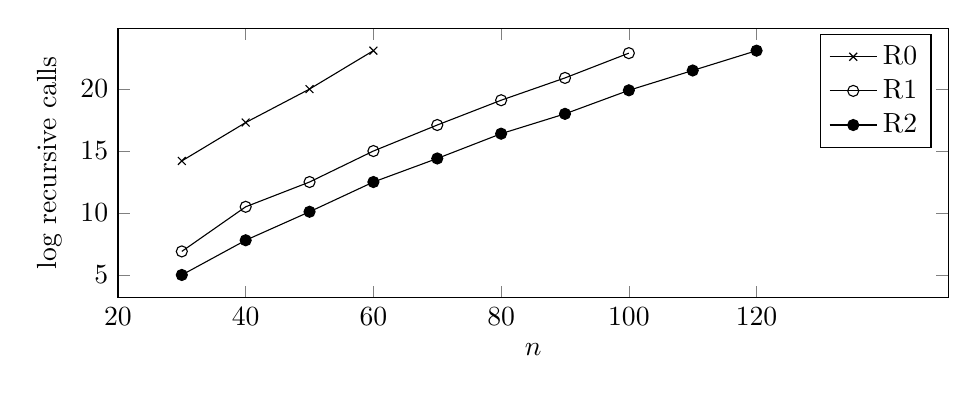
\begin{tikzpicture}
\begin{axis}[
  height= 5cm,
  xlabel=$n$,
  ylabel={log recursive calls},
  xmin = 20,  xmax = 150,
  xtick =       {20,40,60,80,100,120},
  xticklabels = { $20$, $40$, $60$, $80$, $100$, $120$},
  x tick label as interval = false,
  scaled ticks = false
]
    \addplot[color=black, mark=x] 
	coordinates {
	(30, 14.2)
	(40, 17.3)
	(50, 20)
	(60, 23.1)
    };
    \addlegendentry{R0}

    \addplot[color=black, mark=o] 
	coordinates {
	(30, 6.9)
	(40, 10.5)
	(50, 12.5)
	(60, 15)
	(70, 17.1)
	(80, 19.1)
	(90, 20.9)
	(100, 22.9)
    };
    \addlegendentry{R1}

    \addplot[color=black, mark=*] 
	coordinates {
	(30, 5)
	(40, 7.8)
	(50, 10.1)
	(60, 12.5)
	(70, 14.4)
	(80, 16.4)
	(90, 18)
	(100, 19.9)
	(110, 21.5)
	(120, 23.1)
    };
    \addlegendentry{R2}

\end{axis}
\end{tikzpicture}

The running times of algorithm~$R_0$, $R_1$, and $R_2$ appear to be
$O(1.22^n)$, $O(1.17^n)$ and $O(1.15^n)$, respectively.

\subsection{Theoretical Upper Bound}

Denote be $T_i(n)$ the worst runtime of algorithm Ri on \emph{any} graph on $n$ vertices.
Note that $T_i(n)$ is a non-decreasing function of $n$.
For $R_0$ we can conclude that
\begin{align*}
T_0(n) &\leq\max(T_0(n-1), T_0(n-1)+T_0(n-1-d_{\mbox{max}})) \\ &\leq T_0(n-1)+T_0(n-2)
\end{align*}
with $d_{\mbox{max}}$ the degree of the vertex we branch on. The hard part is the one when there are no isolated vertices, in which case the vertex $u$ we are branching on has at least one neighbor. 

For R1 we have that\sidenote{Derive similar recursive bounds on $T_1(n)$ and $T_2(n)$.}
 \[
 T_1(n)=[\ldots]
 \]

For R2 we have that
 \[
 T_2(n)=[\ldots]
 \]
\paragraph{Worst Case Upper Bound}
The running times of algorithm~$R_0$, $R_1$, and $R_2$ are in
$[\ldots],[\ldots],$ and $[\ldots]$, respectively.\sidenote{Replace
  the $[\ldots]$ by a function of $n$ on the form $O(c^n)$.
  Use the recursive bounds you've derived above.
  \emph{Hint: A recurrence of the form $T(n)\leq \sum_{i=1}^k
    a_iT(n-i)$ is called a linear homogeneous recurrence relation with
    constant coefficients.
    To solve it, you can set $T(n)\leq c^n$ where $c$ is the largest
    real root to the characteristic polynomial $x^k-\sum_{i=1}^k
    a_ix^{k-i}$}.}. \newpage
\end{document}
